% Chapter X

\chapter{Pseudo-codice del metodo} % Chapter title

\label{ch:name} % For referencing the chapter elsewhere, use \autoref{ch:name} 
Di seguito verrà proposto lo pseudo-codice dell'algoritmo per il calcolo dell'esposizione al rischio di frana di un \textit{Building}. L'algoritmo qui proposto utilizza un approccio funzionale alla risoluzione del problema: Permette infatti di separare la problematica del calcolo dell'exposure in sotto-problemi atomici. Inoltre ciò semplifica notevolmente la scrittura e la comprensione dello stesso.


% Algorithm

\begin{algorithm}[H]
	
	\SetKwData{Left}{left}\SetKwData{This}{this}\SetKwData{Up}{up}
	\SetKwFunction{Union}{Union}\SetKwFunction{FindCompre
		ss}{FindCompress}
	\SetKwInOut{Input}{Input}\SetKwInOut{Output}{Output}
	
	\IncMargin{1em}
	\Input{$b_i$,$\mathcal{Z}$,$\mathcal{I}$,r,d,l}
	\Output{$exp_i$} 
	\caption{Exposure ($b_i$,$\mathcal{Z}$,$\mathcal{I}$,r,d,l)}
	\label{alg:0}
	\BlankLine
	
	\SetAlgoNoLine
	$ \mathcal{NZ}_i \leftarrow$ NearestZonesFinder($\mathcal{Z},b_i$,r); \\
	$ \mathcal{NI}_i \leftarrow$ NearestIsoipseFinder($\mathcal{I},b_i,r$); \\
	$ \mathcal{ZF}_i \leftarrow$ ZoneFragmentFinder($b_i , \mathcal{NZ}_i, \mathcal{NI}_i $);  \\
	$ \mathcal{BLR}_i \leftarrow $ BufferedLinearRegressionFinder($b_i,\mathcal{ZF}_i,\mathcal{NZ}_i$,d); \\
	$ \mathcal{LS}_i \leftarrow $ LandSlideFinder($b_i , \mathcal{BLR}_i, l$); \\
	$ exp_i \leftarrow$ ContributionOfLandSlide($b_i, \mathcal{LS}_i, l$);\\
	return $ exp_i $;
	
	
\end{algorithm}
La funzione Exposure ($b_i$) elenca i passi fondamentali per poter calcolare il  valore d'exposure dell'edificio $b_i$. Di seguito verranno esposti i dettagli di tutte le funzioni richiamate.

\begin{algorithm}[H]
	
	\SetKwData{Left}{left}
	\SetKwData{This}{this}
	\SetKwData{Up}{up}
	\SetKwFunction{Union}{Union}
	\SetKwFunction{FindCompress}{FindCompress}
	\SetKwInOut{Input}{Input}
	\SetKwInOut{Output}{Output}
	\IncMargin{1em}
	\Input{$\mathcal{Z}$,$b_i$,r}
	\Output{$\mathcal{NZ}_i $} 
	\caption{NearestZonesFinder($\mathcal{Z},b_i$,r)}
	\label{alg:1}
	\BlankLine
	\SetAlgoNoLine
	$ HazardArea_i  \leftarrow $ \textbf{ST\_Buffer($b_i$,r)} ; \\ 
	$ \mathcal{NZ}_i  \leftarrow $ $HazardArea_i \cap \mathcal{Z}$; \\
	return $\mathcal{NZ}_i$;
	
\end{algorithm}

\begin{enumerate}
	\item Crea un buffer ($ HazardArea_i $) di raggio r intorno all'edificio $b_i$
	\item Interseca tale buffer con le zone dell’insieme $\mathcal{Z}$. Il risultato è l’insieme contenente le sole zone con intersezione non vuota con il buffer costruito, ovvero l’insieme  $\mathcal{NZ}_i$
\end{enumerate}

\begin{algorithm}[H]
	
	\SetKwData{Left}{left}\SetKwData{This}{this}\SetKwData{Up}{up}
	\SetKwFunction{Union}{Union}\SetKwFunction{FindCompress}{FindCompress}
	\SetKwInOut{Input}{Input}\SetKwInOut{Output}{Output}
	
	\IncMargin{1em}
	\Input{$\mathcal{I},b_i,r$}
	\Output{$ \mathcal{NI}_i $} 
	\caption{NearestIsoipseFinder($\mathcal{I},b_i,r$)}
	\label{alg:two}
	\BlankLine
	\SetAlgoNoLine
	$  HazardArea_i   \leftarrow $ \textbf{ST\_Buffer($b_i$,r)}; \\
	$ \mathcal{NI}_i \leftarrow $ $HazardArea_i \cap \mathcal{I} $; \\
	return $\mathcal{NI}_i;$
\end{algorithm}
\begin{enumerate}
	\item Crea un buffer ($ HazardArea_i $) di raggio r intorno all'edificio $b_i$
	\item Interseca tale buffer con le isoipse dell’insieme $\mathcal{I}$. Il risultato è l’insieme contenente le sole isoipse con intersezione non vuota con il buffer costruito, ovvero l’insieme  $\mathcal{NI}_i$
\end{enumerate}

\begin{algorithm}[H]
	
	\SetKwData{Left}{left}\SetKwData{This}{this}\SetKwData{Up}{up}
	\SetKwFunction{Union}{Union}\SetKwFunction{FindCompress}{FindCompress}
	\SetKwInOut{Input}{Input}\SetKwInOut{Output}{Output}
	\IncMargin{1em}
	\Input{$b_i,\mathcal{NZ}_i,\mathcal{NI}_i$}
	\Output{$\mathcal{ZF}_i$} 
	\caption{ZoneFragmentFinder($b_i,\mathcal{NZ}_i,\mathcal{NI}_i$)}
	\label{alg:four}
	\BlankLine
	\SetAlgoNoLine
	$\mathcal{ZF}_i \leftarrow$ \O \\
	\For{ each $nz_{i,j}$ in $\mathcal{NZ}_i$  }{
		$Tf$ $\leftarrow$ \O  ; \\
		$Ti$ $\leftarrow nz_{i,j} \cap \mathcal{NI}_i $; \\
		$Tf$ $\leftarrow$ $Tf$ + \textbf{ST\_split($nz_{i,j}$} , $Ti$ [ 1 ] ) ; \\
		$Ti$ $\leftarrow$ $Ti$ - \{ $Ti$ [ 1 ] \}; \\
		\While {Tf is not empty } {
			$Ci$ $\leftarrow $ $Tf$ [ 1 ] $\cap$ $Ti$  ;\\
			\If {Ci is not empty }{
				$Tf$ $\leftarrow$ $Tf$ + \textbf{ST\_split}( $Tf$ [ 1 ], $Ci$ [ 1 ] ) ;\\
				$Tf$ $\leftarrow$ $Tf$ - \{ $Tf$ [ 1 ] \} ;\\
				$Ti$ $\leftarrow$ $Ti$ - \{ $Ci$[ 1 ] \} ;\\
			}
			\Else { 
				$\mathcal{ZF}_i$ $\leftarrow$ $\mathcal{ZF}_i$ + \{ $Tf$ [ 1 ] \} ;\\
				$Tf$ $\leftarrow$ $Tf$ - \{ $Tf$ [ 1 ] \} ;\\
				
			}
		}
	}
	
	return $\mathcal{ZF}_i;$
\end{algorithm}
La funzione ZoneFragmentFinder($b_i$) esegue una multi-split tra $\mathcal{NZ}_i$ e i frammenti di isoipse contenuti nell'insieme $\mathcal{NI}_i$.
Il risultato di detta operazione è descritto in figura \ref{zf}.
\begin{enumerate}
	\item Si inizializza l'insieme $\mathcal{ZF}_i$.
	\item Per ogni $nz_i$ contenuto nell'insieme $\mathcal{NZ}_i$ si attiva l'esecuzione del ciclo. L'indice $i$ è bloccato sul building $i$-esimo mentre la $j$ si muove nell'intervalo (1,..,$\mathbf{card}(\mathcal{NZ}_i)$).
	\item Si inizializza l'insieme $Tf$ (Temp\_fragment) che conterrà i frammenti intermedi prossimi candidati ad essere delle \textit{Zone Fragment} nel caso non ci siano ulteriori split possibili con esse.
	\item Assegnazione all'insieme $Ti$(Temp\_isoipse) del risultato dell'intersezione tra la $nz_{i,j}$ corrente con gli elementi $\mathcal{NI}_i$. Dal punto di vista geometrico ciò equivale a depositare nell'insieme $Ti$ le sole isoipse che interessano la specifica \textit{Nearest Zone}. 
	\item Si esegue lo split della $nz_{i,j}$ con la prima isoipse contenuta nell'insieme $Ti$ che per comodità denoteremo come $Ti$ [1].
	\item Rimozione dell'isoipse $Ti$ [ 1 ] usata nella split precedente, poichè essendo già stata usata per una split non potrà produrne altre.
	\item Se $Tf \not=\emptyset$ allora esistono ancora frammenti intermedi che potrebbero essere splittati dalle rimanenti isoipse.
	\item Si interseca il primo frammento di $Tf$, che per comodità denoteremo con $Tf$ [ 1 ], con le rimanenti isoipse $Ti$. Il risultato genera un nuovo insieme chiamato $Ci$(Current\_isoipses).
	\item Se l'insieme $Ci \not=\emptyset$, vuol dire che il frammento $Tf$ [ 1 ] è ulteriormente splittabile in quanto intersecato da almeno una isoipse.
	\\
	Se invece $Ci =\emptyset$, risulta che il frammento non è attraversato da nessuna isoipse, per cui non sarà più splittabile.
	\item Viene eseguito lo split di $Tf$ [1] con il (frammento) di isoipse $Ci$[1] ed il risultato viene aggiunto all'insieme $Tf$.
	\item Rimozione del frammento $Tf$ [1] dall'insieme $Tf$ poichè è stato precedentemente splittato in sotto frammenti.
	\item Rimozione della isoipse che ha prodotto lo split ovvero $Ci$ [i].
\end{enumerate}
\begin{enumerate}
	\setcounter{enumi}{14}
	\item Aggiunta del framento $Tf$ [ 1 ] all'insieme $\mathcal{ZF}_i$  poichè non risulta più splittabile.
	\item Rimozione del frammento $Tf$ [ 1 ] dall'insieme $Tf$ essendo ormai elemento dell'insieme dei frammenti atomici non più splittabili.
\end{enumerate}
\begin{enumerate}
		\setcounter{enumi}{19}
		\item Viene restituito l'insieme $\mathcal{ZF}_i$
\end{enumerate}

Per agevolare la comprensione dell'algoritmo viene ora proposto un esempio 
illustrativo. Supponiamo di avere una nearest zone e delle nearest isoipses come in figura \ref{pseudo1}. 

\begin{figure}[h]
	\centering
	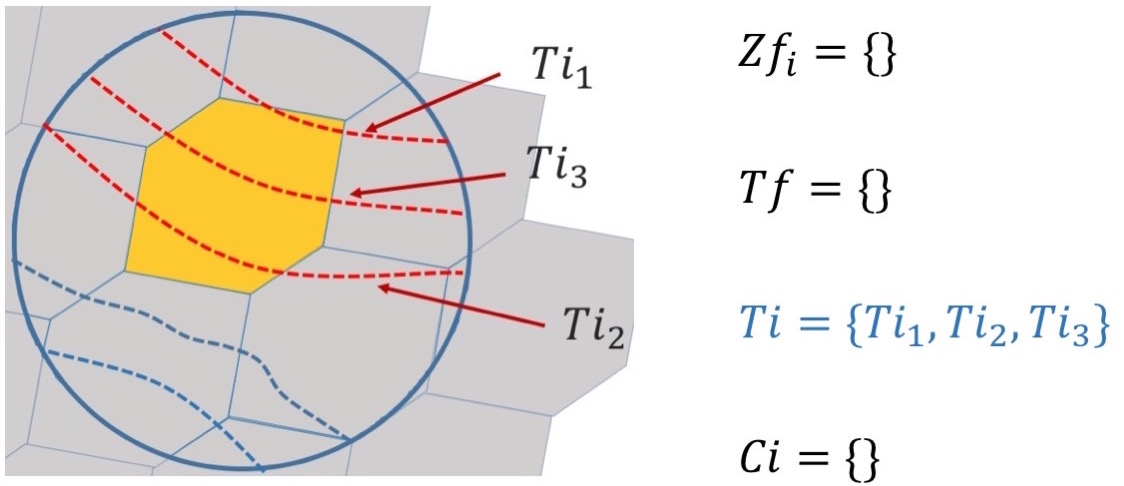
\includegraphics[width=0.6\textwidth]{images/pseudo1}
	\caption{}
	\label{pseudo1}
\end{figure}

Eseguendo la riga 4 dello pseudo codice  all'array $Ti$ verranno aggiunte le $ni_{i,o}$ che intersecano la $nz_{i,j}$ (di colore arancione) $Ti_1$, $Ti_2$, $Ti_3$ (di colore rosso). 
A questo punto viene eseguita la riga 5 che splitta la $nz_{i,j}$ con la prima isoipse dell'array $Ti$. Il risultato sono due geometrie che chiameremo $Tf_1$ e $Tf_2$ (Figura \ref{pseudo2}) che vengono aggiunte nell'insieme $Tf$. La nearest isoipse $Ti_1$ è stata utilizzata e quindi viene rimossa dall'array.
	
\begin{figure}[h]
	\centering
	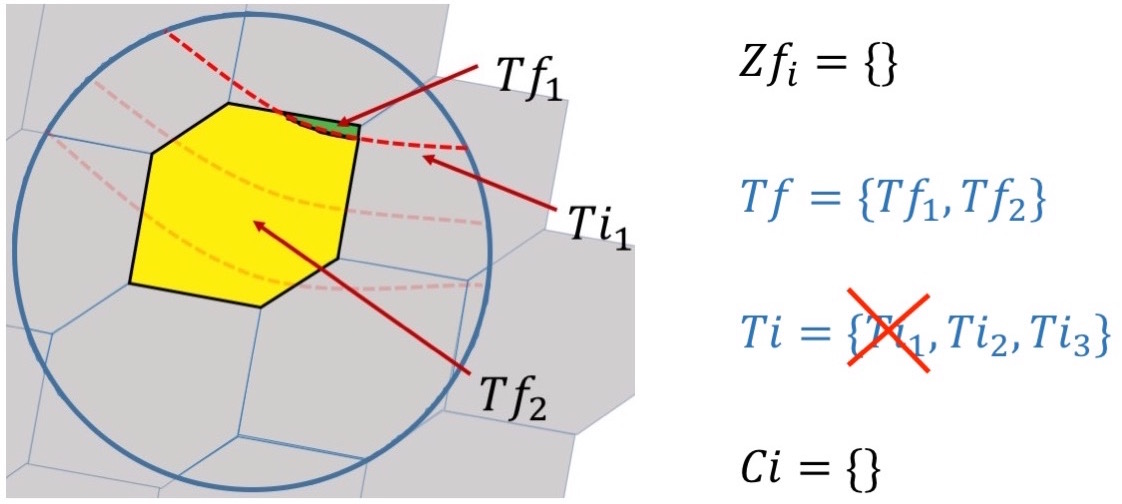
\includegraphics[width=0.6\textwidth]{images/pseudo2}
	\caption{}
	\label{pseudo2}
\end{figure}

A questo punto si verifica, con la condizione del ciclo while alla riga 7, se l'insieme $Tf$ è non vuoto. In questo esempio la condizione è verificata e quindi si entra nel ciclo. Il primo elemento dell'array $Tf$ è $Tf_1$ che non interseca nessuna $ni_{i,o}$ dell'array $Ti$ (Figura \ref{pseudo3}). Quindi l'array $Ci$ della riga 8 è vuoto. Ciò comporta che nell'istruzione succesiva la condizione $Ci$ "non vuoto" non è verificata. Si esegue quindi il ramo else della riga 14. Il primo elemento di $Tf$ viene spostato dall'insieme $ZF_i$.

\begin{figure}[h]
	\centering
	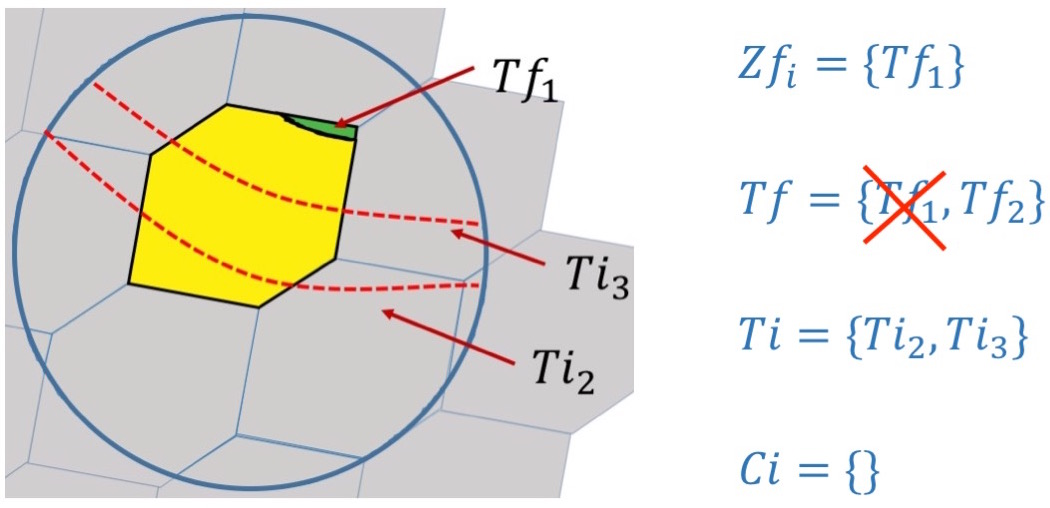
\includegraphics[width=0.6\textwidth]{images/pseudo3}
	\caption{}
	\label{pseudo3}
\end{figure}

Si ritorna quindi alla riga 7. La condizione del while è verificata in quanto  $Tf$ contiene $Ti_2$. Quest'ultima viene interseca sia $Ti_2$ e $Ti_3$ è quindi l'array $Ci$ conterrà i due elementi (riga 8). Di conseguenza la condizione sulla riga 9 è verificata e quindi $Tf_2$ viene splittato con il primo elemento di $Ci$ ovvero $Ti_2$. Vengono create quindi due nuove geometrie $Tf_3$ e $Tf_4$ (Figura \ref{pseudo4}) e vengono aggiunte all'array $Tf$. Da quest'ultimo viene tolta $Tf_2$. Da $Ti$ viene rimossa $Ti_2$.
	
\begin{figure}[h]
	\centering
	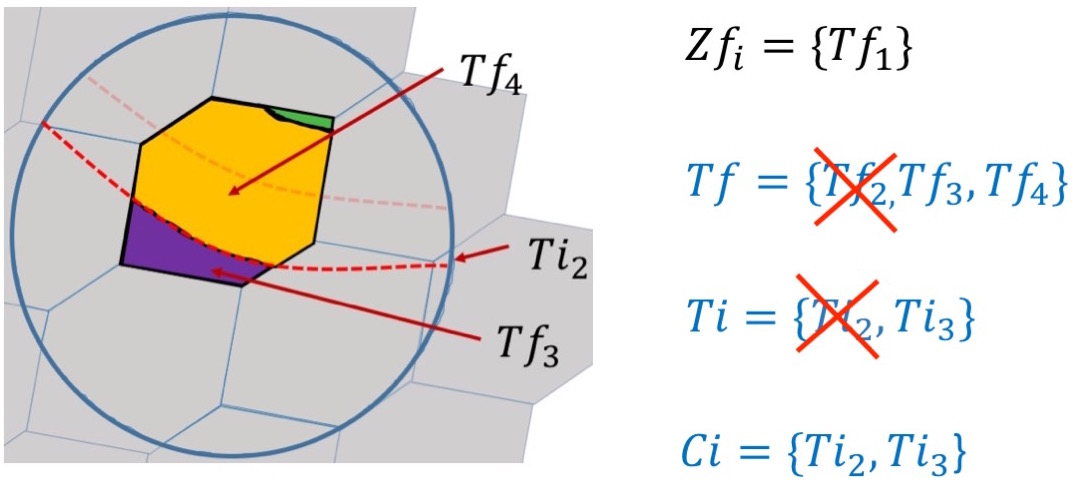
\includegraphics[width=0.6\textwidth]{images/pseudo4}
	\caption{}
	\label{pseudo4}
\end{figure}

Si ritorna alla riga 7. $Tf$ non è vuoto (contiene $Tf_3$ e $Tf_4$). $Tf_3$ non interseca con $Ti_3$ (Figura \ref{pseudo5}) motivo per cui $Ci$ è vuoto. Quindi viene eseguito il ramo else dell'if alla riga 14. $Tf_3$ viene aggiunto all'array $Zf_i$ e all'istruzione successiva rimosso dall'array $Tf$.
	
\begin{figure}[h]
	\centering
	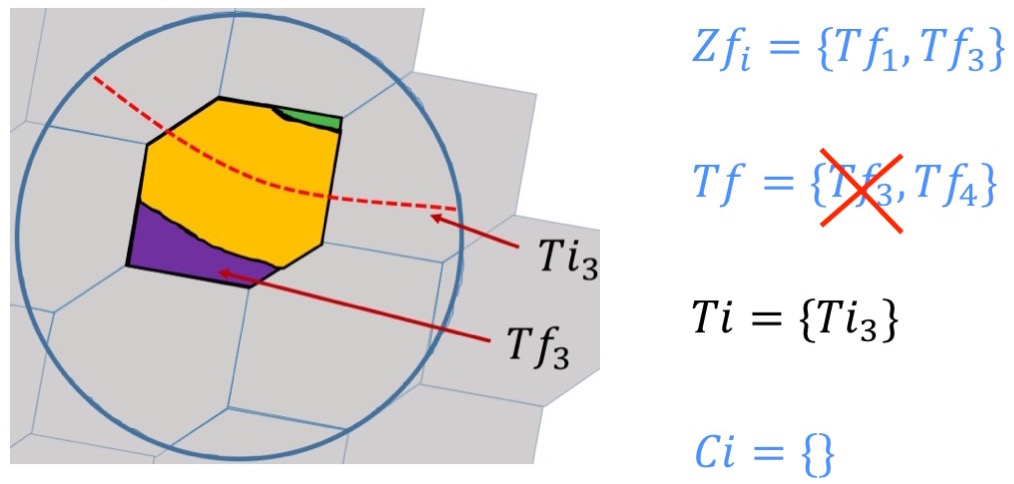
\includegraphics[width=0.6\textwidth]{images/pseudo5}
	\caption{}
	\label{pseudo5}
\end{figure}

Di nuovo si torna alla riga 7. $Tf$ non è vuoto, contiene $Tf_4$ che interseca con la $Ti_3$. Quindi $Ci$ è non vuoto e $Tf_4$ viene splittato con $Ti_3$. Il risultato dell'operazione, le geometrie $Tf_5$ e $Tf_6$, vengono aggiunte all'array $Tf$ (Figura \ref{pseudo6}). $Tf_4$ viene rimosso da $Tf$ e $Ti_3$ da $Ti$. 

\begin{figure}[h]
	\centering
	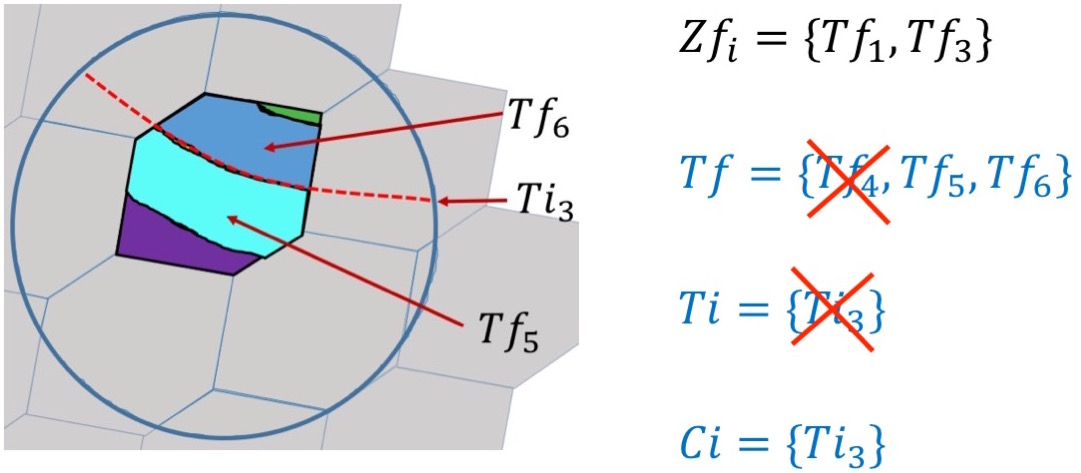
\includegraphics[width=0.6\textwidth]{images/pseudo6}
	\caption{}
	\label{pseudo6}
\end{figure}

Arrivato a questo punto l'array $Ti$ non ha più elementi. Quindi l'intersezione tra $Tf_5$ ( e successivamente $Tf_6$ ) con $Ti$ alla riga 8 risulterà nulla. Per questo motivo $Ci$ è vuoto e viene eseguita la riga 14 (Figura \ref{pseudo7}).

\begin{figure}[h]
	\centering
	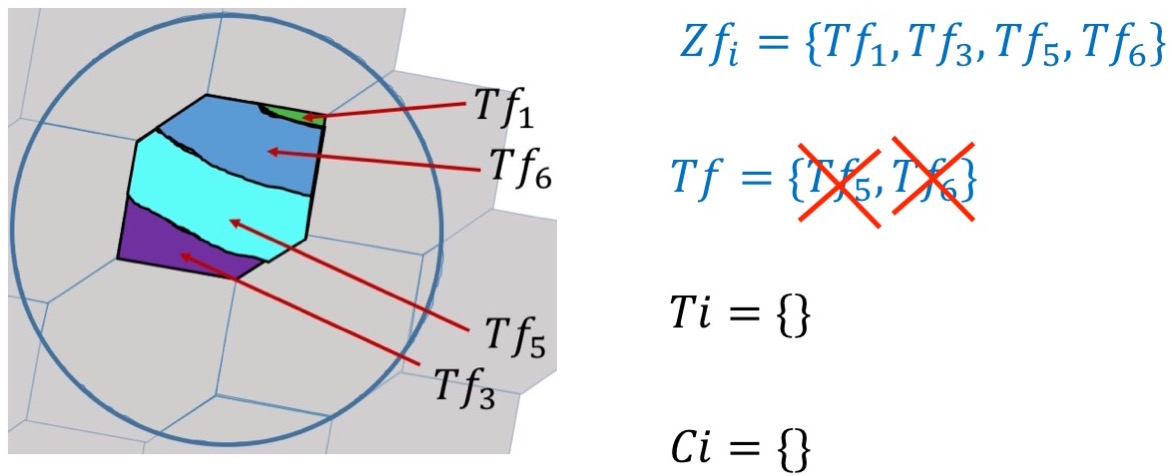
\includegraphics[width=0.6\textwidth]{images/pseudo7}
	\caption{}
	\label{pseudo7}
\end{figure}

Per finire $Tf$ è un array vuoto quindi la condizione del while alla riga 7 non è più verificata. L'algoritmo termina è ritorna l'array $Zf_i$ contenete i zone fragments.

\newpage
	

\begin{algorithm}[H]
	
	\SetKwData{Left}{left}\SetKwData{This}{this}\SetKwData{Up}{up}
	\SetKwFunction{Union}{Union}\SetKwFunction{FindCompress}{FindCompress}
	\SetKwInOut{Input}{Input}\SetKwInOut{Output}{Output}
	\IncMargin{1em}
	\Input{$b_i,\mathcal{ZF}_i,\mathcal{NZ}_i$,d}
	\Output{$\mathcal{BLR}_i$} 
	\caption{BufferedLinearRegressionFinder($b_i , \mathcal{ZF}_i , \mathcal{NZ}_i$,d)}
	\label{alg:four}
	\BlankLine
	\SetAlgoNoLine
	$\mathcal{BLR}_i \leftarrow$ \O ;\\
	\For {$nz_{i,j}$ in $\mathcal{NZ}_i$}{
		$cnz_{i,j} \leftarrow$ \textbf{ST\_centroid}($nz_{i,j}$) ;\\
		\For {($zf_{i,j,t} \in \mathcal{ZF}_i) \subset nz_{i,j}$ }{
			$Cp$ $\leftarrow$ $Cp$ + \{\textbf{ST\_centroid}($zf_{i,j,t}$) \} ;\\
		}
		$slope$ $\leftarrow$ \textbf{regr\_slope}($Cp$) ;\\
		$lr_{i,j}$ $\leftarrow$ \textbf{ST\_MakeLine}($slope$,$cnz_{i,j}$) ;\\
		$\mathcal{BLR}_i \leftarrow \mathcal{BLR}_i $ + \{(\textbf{ST\_Buffer}($lr_{i,j}$,d)) \} ;\\
	}
	
	return $\mathcal{BLR}_i;$
	
\end{algorithm}

\begin{enumerate}
	\item Si inizializza l'insieme $\mathcal{BLR}_i$.
	\item Per ogni elemento all'interno dell'insieme $\mathcal{NZ}_i$ si attiva il ciclo for. L'indice $i$ è bloccato sul building $i$-esimo mentre la $j$ si muove nell'intervalo (1,..,$\mathbf{card}(\mathcal{NZ}_i)$).
	\item Calcolo del centroide $cnz_{i,j}$.
	\item Per ogni $zf_{i,j,t}$ contenuto in $nz_i$ si attiva il secondo ciclo for (figura \ref{zf}) 
	\item Calcolo dei centroidi di $zf_{i,j,t}$ ed inserimento dei punti risultanti in un insieme chiamato Cp(Centroid\_point) (Figura \ref{czf})
\end{enumerate}
\begin{enumerate}
	\setcounter{enumi}{6}
	\item Calcolo della pendenza della retta di regressione lineare sull'insieme dei punti $Cp$ con la primitiva di Postgres "regr\_slope" ed assegnazione del risultato alla variabile chiamata "$slope$"
	\item Calcolo della retta $lr_{i,j}$ passante per il punto $cnz_{i,j}$ e avente coefficiente angolare pari a "$slope$".
	\item Aggiunta a $\mathcal{BLR}_i$ del risultato della \textit{LineBuffering} della retta $lr_{i,j}$.
\end{enumerate}
\begin{enumerate}
	\setcounter{enumi}{10}
	\item Viene restituito l'insieme $\mathcal{BLR}_i$
\end{enumerate}


\begin{algorithm}[H]
	
	\SetKwData{Left}{left}\SetKwData{This}{this}\SetKwData{Up}{up}
	\SetKwFunction{Union}{Union}\SetKwFunction{FindCompress}{FindCompress}
	\SetKwInOut{Input}{Input}\SetKwInOut{Output}{Output}
	\IncMargin{1em}
	\Input{$b_i, \mathcal{BLR}_i, l$}
	\Output{$\mathcal{LS}_i$} 
	\caption{LandSlideFinder($b_i , \mathcal{BLR}_i, l$) }
	\label{alg:four}
	\BlankLine
	\SetAlgoNoLine
	$ BuildingBuffer_i  \leftarrow $ \textbf{ST\_Buffer($b_i$,l)} ;\\
	$ \mathcal{LS}_i \leftarrow $ \textbf{ST\_intersection}($BuildingBuffer_i,\mathcal{BLR}_i $) ;\\
	return $\mathcal{LS}_i;$
\end{algorithm}

\begin{enumerate}
	\item Si crea un buffer di raggio $d$ intorno all'edificio $b_i$
	\item Si interseca il buffer appena creato con l'insieme  $\mathcal{BLR}_i$
	\item Ne Risulta un insieme contenente le sole $\mathcal{BLR}_i$ intersecate al buffer.(figura \ref{landslides}) 
\end{enumerate}

\begin{algorithm}[H]
	
	\SetKwData{Left}{left}\SetKwData{This}{this}\SetKwData{Up}{up}
	\SetKwFunction{Union}{Union}\SetKwFunction{FindCompress}{FindCompress}
	\SetKwInOut{Input}{Input}\SetKwInOut{Output}{Output}
	\IncMargin{1em}
	\Input{$b_i, \mathcal{LS}_i ,\mathcal{LSZ}_i, d $}
	\Output{$exp_i$} 
	\caption{ContributionOfLandSlide($b_i , \mathcal{LS}_i, \mathcal{LSZ}_i, l $) }
	\label{alg:four}
	\BlankLine
	\SetAlgoNoLine
	
	$ exp_i \leftarrow$ \O ;\\
	$ BuildingBuffer_i  \leftarrow $ \textbf{ST\_Buffer($b_i$, l)} ;\\
	\For { each $  ls_{i,j} \in \mathcal{LS}_i $ }{
		\If{\textbf{ST\_intersects($b_i, lsz_{i,j}$)}}{
			$exp_i \leftarrow $ $exp_i$ + $pexp_{i,j}$ ($equation$ \ref{eq:exposure3}) ;\\
		}
		\Else {
			$exp_i \leftarrow $ $exp_i$ + $pexp_{i,j}$ ($equation$ \ref{eq:exposure2}) ;\\
		}
		
	}
	return $exp_i;$
\end{algorithm}
La funzione ContributionOfLandSlide($b_i , \mathcal{LS}_i, \mathcal{LSZ}_i, l $) somma tutti i contributi delle \textbf{Landslide} che impattano sull'edificio.
\begin{enumerate}
	\item Si inizializza la variabile $exp_i$ 
	\item Si calcola il buffer di raggio $l$ intorno al building $i$-esimo
	\item Per ogni elemento $ls_{i,j}$ contenuto in $\mathcal{LS}_i $ si avvia il ciclo for.
	\item Se l'intersezione tra ($ls_{i,j}$ con $b_i$)$\not=\emptyset$, allora la $ls_{i,j}$ del corrente ciclo corrisponde alla	\textit{LandSlide} ove è ubicato il building.\\
	Altrimenti la $ls_{i,j}$ corrisponde ad una \textit{LandSlide} che non contiene il building. 
	\item Si calcola il valore di \textit{Partial Exposure} con l'equazione \ref{eq:exposure3}) a ed il risultato viene sommato a $exp_i$.
\end{enumerate}
\begin{enumerate}
	\setcounter{enumi}{7}
	\item Si calcola il valore di \textit{Partial Exposure} con l'equazione \ref{eq:exposure2} ed il risultato viene sommato a $exp_i$. 
\end{enumerate}
\begin{enumerate}
	\setcounter{enumi}{10}
	\item Viene restituito il valore di exposure totale del building $i$-esimo
\end{enumerate}
